% Bài báo NCKH - template SSRC (IEEEtran) trên Overleaf
% Ảnh cần upload cùng main.tex: hinh-5-2-calibration.png, sla_nhan_biet.png, roc_tiep_nhan.png, roc_tham_dinh.png, nguong_tiep_nhan.png, nguong_tham_dinh.png
\documentclass[journal]{IEEEtran}
\usepackage[utf8]{vietnam}

\usepackage{cite}
\usepackage{amsmath,amssymb,amsfonts}
\usepackage{graphicx}
\usepackage{tikz}
\usetikzlibrary{positioning,arrows.meta}
\usepackage{textcomp,nicefrac}
\def\BibTeX{{\rm B\kern-.05em{\sc i\kern-.025em b}\kern-.08em
    T\kern-.1667em\lower.7ex\hbox{E}\kern-.125emX}}


\markboth{STUDENT SCIENTIFIC RESEARCH COMMUNICATION, VOLUME I, 2026}{STUDENT SCIENTIFIC RESEARCH COMMUNICATION, VOLUME I, 2026}

\begin{document}

\title{Tích hợp mô hình dự báo nguy cơ trễ hạn xử lý vào hệ thống quản lý quy trình vay vốn doanh nghiệp nhỏ và vừa}

\author{Voòng Thị Yến Trang, Lê Thị Yến Nhi, Ngô Hữu Dũng*\\
Khoa Công nghệ Thông tin, Trường Đại học Công nghiệp TP. HCM\\
voongtrang4107@gmail.com, yenjj2025@gmail.com, *ngohuudung@iuh.edu.vn}

\maketitle

{\renewcommand{\abstractname}{Abstract}
\begin{abstract}
Loan applications of small and medium-sized enterprises pass through several processing stages, and each stage has a deadline, called the service-level agreement, measured in working hours. Branch managers cannot monitor every application, and conventional systems mark a case as overdue only after the deadline has passed. This paper presents a loan workflow system that integrates a delay-risk predictor as a separate service. Two models, one for each stage, estimate the probability that an open application will exceed its deadline. The deadline is an input of the models, so a new deadline can be applied without retraining; the probabilities are calibrated by isotonic regression, and each alert carries at most three reasons. The models are trained on 20,000 simulated applications whose waiting-time distributions follow a public loan-application event log. On a held-out set, the area under the receiver operating characteristic curve reaches 0.824 for the intake stage (0.813 on average over five random splits) and 0.720 for the appraisal stage, against 0.797 and 0.687 for a baseline that only knows the deadline clock. The gain is statistically clear for appraisal but not for intake, where only 38 late cases are available. Treating the deadline as an input keeps probabilities accurate when the deadline changes, whereas a model trained at one fixed deadline does not. The results were reproduced exactly on an independent cloud environment. Because the data are simulated, they describe the method and not the performance on real bank data.
\end{abstract}

\begin{IEEEkeywords}
Loan processing, predictive process monitoring, probability calibration, service-level agreement.
\end{IEEEkeywords}}

\begin{abstract}
Hồ sơ vay của doanh nghiệp nhỏ và vừa đi qua nhiều công đoạn, mỗi công đoạn có một hạn xử lý chuẩn tính bằng giờ làm việc. Các hệ thống thông thường chỉ báo hồ sơ quá hạn sau khi đã trễ. Bài báo trình bày hệ thống quản lý quy trình vay tích hợp bộ dự báo nguy cơ trễ dưới dạng một dịch vụ riêng. Hai mô hình, mỗi công đoạn một mô hình, ước lượng xác suất hồ sơ đang mở sẽ vượt hạn xử lý. Hạn xử lý là đầu vào của mô hình nên đổi định mức không cần huấn luyện lại; xác suất được hiệu chỉnh bằng hồi quy đẳng điệu và mỗi cảnh báo kèm tối đa ba lý do. Mô hình huấn luyện trên 20\,000 hồ sơ mô phỏng theo một nhật ký xử lý hồ sơ vay công khai. Trên tập kiểm tra, diện tích dưới đường cong đặc trưng hoạt động của bộ thu nhận đạt 0,824 ở tiếp nhận (trung bình năm lần chia dữ liệu là 0,813) và 0,720 ở thẩm định, so với 0,797 và 0,687 của đường cơ sở chỉ biết đồng hồ hạn xử lý. Mức cải thiện có ý nghĩa thống kê ở thẩm định nhưng chưa đủ bằng chứng ở tiếp nhận, nơi chỉ có 38 hồ sơ trễ. Mô hình huấn luyện ở một hạn cố định mất độ chính xác xác suất khi đổi hạn, còn mô hình nhận hạn làm đầu vào thì không. Kết quả được tái lập trên một môi trường độc lập. Do dữ liệu mô phỏng, kết quả chỉ phản ánh phương pháp.
\end{abstract}

\begin{IEEEkeywords}
Doanh nghiệp nhỏ và vừa, dự báo trễ hạn, hiệu chỉnh xác suất, quy trình vay vốn.
\end{IEEEkeywords}

% ============================================================
\section{Giới thiệu}
% ============================================================
Hồ sơ vay vốn của doanh nghiệp nhỏ và vừa (SME) tại một chi nhánh ngân hàng được xử lý tuần tự qua nhiều công đoạn, chẳng hạn tiếp nhận và rà soát chứng từ, thẩm định và phê duyệt. Mỗi công đoạn có một hạn xử lý chuẩn (SLA, service-level agreement) tính bằng giờ làm việc của ngân hàng. Khi hồ sơ vượt SLA, doanh nghiệp phải chờ lâu hơn và chi nhánh bị đánh giá thấp về chất lượng phục vụ.

Ở chi nhánh nhỏ, số cán bộ ít nhưng mỗi người đồng thời giữ nhiều hồ sơ, nên quản lý khó biết hồ sơ nào đang có nguy cơ trễ. Các hệ thống quản lý quy trình thông thường chỉ đánh dấu ``quá hạn'' sau khi hồ sơ đã vượt SLA, lúc đó việc can thiệp đã muộn. Điều quản lý cần là một cảnh báo sớm, đủ tin cậy để quyết định giao lại hay đẩy nhanh hồ sơ, và nằm ngay trong luồng làm việc hằng ngày thay vì một báo cáo tách rời. Cảnh báo này chỉ phục vụ điều phối, không chấm điểm tín dụng và không thay quyết định phê duyệt của con người.

Bài báo trình bày một hệ thống quản lý quy trình vay SME có tích hợp dự báo nguy cơ trễ SLA. Đóng góp gồm:
\begin{itemize}
\item Một hệ thống gồm giao diện, máy chủ nghiệp vụ và dịch vụ dự báo tách rời; khi dịch vụ dự báo ngừng hoạt động, nghiệp vụ vay vẫn chạy bình thường.
\item Giải pháp dự báo theo từng công đoạn, nhận SLA làm đầu vào để đổi định mức không phải huấn luyện lại, có hiệu chỉnh xác suất và lý do giải thích kèm theo.
\item Quy trình tích hợp được kiểm chứng: thời điểm kích hoạt dự báo, quy tắc hiển thị, kiểm thử tự động và kiểm chứng trên hệ thống đang chạy.
\end{itemize}

Phần còn lại của bài báo được tổ chức như sau. Mục~II điểm lại các nghiên cứu liên quan, Mục~III trình bày cơ sở lý thuyết, Mục~IV mô tả kiến trúc hệ thống, Mục~V mô tả dữ liệu và mô hình, Mục~VI trình bày thực nghiệm, Mục~VII nêu các hạn chế và Mục~VIII kết luận.

% ============================================================
\section{Nghiên cứu liên quan}
% ============================================================
\subsection{Giám sát quy trình có dự báo}
Dự báo kết quả hoặc thời gian còn lại của một ca đang chạy từ nhật ký sự kiện là một hướng nghiên cứu của khai phá quy trình, thường gọi là giám sát quy trình có dự báo. Teinemaa và cộng sự khảo sát các phương pháp dự báo theo kết quả, xây dựng phân loại các phương pháp và so sánh thực nghiệm giữa chúng \cite{teinemaa2019}. Verenich và cộng sự thực hiện công việc tương tự cho bài toán dự báo thời gian còn lại \cite{verenich2019}. Các nghiên cứu này tập trung vào việc so sánh thuật toán trên nhiều nhật ký sự kiện công khai. Bài báo này quan tâm đến một khía cạnh khác: đưa bộ dự báo vào một hệ thống nghiệp vụ đang chạy, trong đó SLA là tham số do quản trị viên thay đổi được và dự báo phải gắn với đúng công đoạn của hồ sơ.

\subsection{Dự báo thời gian chờ và hàng đợi}
Tax và cộng sự dùng mạng nơ-ron LSTM để dự báo hoạt động kế tiếp và thời gian còn lại của ca đang chạy \cite{tax2017}. Senderovich và cộng sự cho thấy đặc trưng về hàng đợi (số ca đang chờ cùng lúc, loại yêu cầu) cải thiện rõ rệt dự báo độ trễ so với các bộ dự báo bỏ qua hàng đợi \cite{senderovich2015}. Bài báo này kế thừa ý tưởng đó khi đưa độ dài hàng chờ và tải cán bộ vào đặc trưng vận hành, và bóc tách ở Mục~VI cho thấy nhóm đặc trưng này đóng góp phần lớn sức dự báo.

\subsection{Xác suất tin cậy}
Khi người dùng đọc trực tiếp con số dự báo như một xác suất, con số này phải phản ánh đúng tần suất thực tế. Niculescu-Mizil và Caruana chỉ ra rằng đầu ra của các phương pháp như cây tăng cường thường bị đẩy ra xa 0 và 1, và có thể được sửa bằng hiệu chỉnh Platt hoặc hồi quy đẳng điệu; họ cũng lưu ý hồi quy đẳng điệu dễ quá khớp khi dữ liệu hiệu chỉnh ít \cite{niculescu2005}. Guo và cộng sự chỉ ra rằng các mạng nơ-ron sâu hiện đại cũng thường dự báo xác suất kém tin cậy \cite{guo2017}. Bài báo này dùng hồi quy đẳng điệu vì tập kiểm định đủ lớn (hơn mười nghìn dòng mỗi công đoạn) và đánh giá độ tin cậy bằng điểm Brier \cite{brier1950}.


% ============================================================
\section{Cơ sở lý thuyết}
% ============================================================
\subsection{Phát biểu bài toán}
Gọi $S$ là SLA của công đoạn (giờ làm việc), $e$ là số giờ làm việc hồ sơ đã dùng ở công đoạn đó, $x$ là vector đặc trưng của hồ sơ và tình trạng vận hành, và $T$ là tổng số giờ công đoạn sẽ tiêu tốn khi kết thúc. Số giờ đã dùng được tính theo lịch làm việc của ngân hàng và trừ thời gian chờ doanh nghiệp:
\begin{equation}
e=W(t_0,t)-P(t_0,t),
\end{equation}
trong đó $t_0$ là lúc hồ sơ vào công đoạn, $t$ là thời điểm dự báo, $W$ là số giờ làm việc trong khoảng $[t_0,t]$ và $P$ là số giờ đồng hồ SLA tạm dừng vì chờ doanh nghiệp bổ sung. Tại thời điểm hồ sơ còn mở và chưa quá hạn ($e<S$), cần ước lượng
\begin{equation}
p=\Pr(T>S\mid x,e,S).
\end{equation}
Đây là bài toán phân loại nhị phân với nhãn $y=\mathbb{1}[T>S]$. Số giờ còn lại là
\begin{equation}
r=S-e.
\end{equation}
Hồ sơ có $e\ge S$ đã quá hạn, là sự việc đã xảy ra và được xác định bằng quy tắc tất định (Mục~IV-D), không cần mô hình.

\subsection{Các thuật toán phân loại}
Gọi $\mathbf{z}$ là vector đặc trưng đã mã hóa, gồm $x$, $e$, $S$ và $r$. Hồi quy logistic ước lượng xác suất bằng hàm sigmoid $\sigma(u)=1/(1+e^{-u})$ của một tổ hợp tuyến tính các đặc trưng:
\begin{equation}
p=\sigma(\mathbf{w}^{\top}\mathbf{z}+b);
\end{equation}
nó đơn giản và dễ giải thích. Gradient Boosting \cite{friedman2001} cộng dần nhiều cây quyết định nhỏ $h_m$, mỗi cây mới sửa phần sai của các cây trước, nên bắt được quan hệ phi tuyến giữa các đặc trưng:
\begin{equation}
F_m(\mathbf{z})=F_{m-1}(\mathbf{z})+\nu\,h_m(\mathbf{z}),\qquad p=\sigma\bigl(F_M(\mathbf{z})\bigr),
\end{equation}
với tốc độ học $\nu=0{,}06$ và tối đa $M=400$ cây. Cả hai được cài đặt trong scikit-learn \cite{pedregosa2011}; Gradient Boosting dùng biến thể dựa trên histogram để huấn luyện nhanh. Các thuật toán được so sánh bằng hàm mất mát log-loss trên $N$ mẫu:
\begin{equation}
\mathcal{L}=-\frac{1}{N}\sum_{i=1}^{N}\bigl[y_i\ln p_i+(1-y_i)\ln(1-p_i)\bigr],
\end{equation}
giá trị càng nhỏ thì xác suất dự báo càng sát nhãn thật.

\subsection{Hiệu chỉnh xác suất}
Đầu ra của bộ phân loại chưa chắc là xác suất đúng nghĩa: điểm số 0,6 chưa chắc ứng với 60\% hồ sơ thực sự trễ. Gọi $s_i$ là điểm số thô của dòng $i$ trên tập kiểm định. Hồi quy đẳng điệu (isotonic regression) học một hàm không giảm biến điểm số thành xác suất sao cho sai số bình phương nhỏ nhất \cite{niculescu2005}:
\begin{equation}
\hat{g}=\operatorname*{arg\,min}_{g\ \text{không giảm}}\ \sum_{i}\bigl(y_i-g(s_i)\bigr)^2,\qquad \hat{p}=\hat{g}(s).
\end{equation}
Vì chỉ yêu cầu hàm không giảm, phương pháp không giả định dạng hàm cụ thể và giữ nguyên thứ tự xếp hạng của điểm số.

\subsection{Chỉ số đánh giá}
Diện tích dưới đường cong đặc trưng hoạt động của bộ thu nhận (ROC), viết tắt là AUC, là xác suất một hồ sơ trễ được chấm điểm cao hơn một hồ sơ đúng hạn chọn ngẫu nhiên; 0,5 ứng với đoán bừa và 1 là hoàn hảo:
\begin{equation}
\mathrm{AUC}=\Pr\bigl(s^{+}>s^{-}\bigr)+\tfrac{1}{2}\Pr\bigl(s^{+}=s^{-}\bigr),
\end{equation}
với $s^{+}$ và $s^{-}$ là điểm của một hồ sơ trễ và một hồ sơ đúng hạn chọn ngẫu nhiên. Điểm Brier \cite{brier1950} là trung bình bình phương sai số giữa xác suất dự báo và nhãn, nhỏ hơn thì tốt hơn và được so với mức đoán theo tỷ lệ trễ chung:
\begin{equation}
\mathrm{Brier}=\frac{1}{N}\sum_{i=1}^{N}(p_i-y_i)^2.
\end{equation}
Sai số hiệu chỉnh kỳ vọng (ECE) chia các dòng thành $M$ nhóm theo xác suất dự báo và lấy độ chênh trung bình có trọng số giữa xác suất dự báo và tỷ lệ trễ thực tế của từng nhóm $B_m$; nhỏ hơn thì xác suất đáng tin hơn:
\begin{equation}
\mathrm{ECE}=\sum_{m=1}^{M}\frac{|B_m|}{N}\,\bigl|\,\overline{y}(B_m)-\overline{p}(B_m)\,\bigr|.
\end{equation}
Khi chuyển xác suất thành cảnh báo theo ngưỡng, dùng độ chính xác (phần cảnh báo đúng), độ phủ (phần hồ sơ trễ được cảnh báo) và tỷ lệ báo nhầm (phần hồ sơ đúng hạn bị cảnh báo), tính từ số cảnh báo đúng (TP), cảnh báo sai (FP), hồ sơ trễ bị bỏ sót (FN) và hồ sơ đúng hạn không bị cảnh báo (TN):
\begin{equation}
\text{Chính xác}=\frac{TP}{TP+FP},\quad \text{Phủ}=\frac{TP}{TP+FN},\quad \text{Báo nhầm}=\frac{FP}{FP+TN}.
\end{equation}

\subsection{Giải thích lý do cảnh báo}
Để chỉ ra yếu tố nào đẩy xác suất lên, bài báo thay lần lượt giá trị của từng yếu tố $j$ bằng giá trị điển hình $\tilde{x}_j$ (trung vị trên dữ liệu huấn luyện) và đo mức giảm xác suất:
\begin{equation}
\Delta_j=p(x)-p\bigl(x^{(j\leftarrow\tilde{x}_j)}\bigr).
\end{equation}
Những yếu tố có $\Delta_j\ge 0{,}05$ được nêu làm lý do, tối đa ba yếu tố. Đây là giải thích về cách mô hình dựa vào đặc trưng, không chứng minh quan hệ nhân quả ngoài thực tế.

% ============================================================
\section{Kiến trúc hệ thống}
% ============================================================
\subsection{Tổng quan}
Hệ thống gồm ba thành phần chạy độc lập, giao tiếp qua HTTP và đóng gói bằng Docker Compose (Hình~\ref{fig:arch}): giao diện web viết bằng React và TypeScript; máy chủ nghiệp vụ viết bằng NestJS với Prisma, lưu dữ liệu trong PostgreSQL; và dịch vụ dự báo viết bằng Python, FastAPI và scikit-learn. Dịch vụ dự báo được tách riêng vì các thư viện học máy trưởng thành nhất nằm ở hệ sinh thái Python, trong khi nghiệp vụ viết bằng TypeScript; cách tách này còn giúp hệ thống chịu lỗi, vì khi dịch vụ dự báo tắt thì nghiệp vụ vay vẫn chạy và lỗi chỉ được ghi nhật ký.

\begin{figure}[t]
\centering
\begin{tikzpicture}[node distance=0.6cm and 0.9cm,
  box/.style={draw,rounded corners=2pt,align=center,font=\footnotesize,minimum width=2.6cm,minimum height=0.9cm},
  arr/.style={-{Stealth[length=5pt]},thick}]
\node[box] (ui) {Giao diện\\React + TypeScript};
\node[box,right=of ui] (api) {Máy chủ nghiệp vụ\\NestJS + Prisma};
\node[box,below=of api] (ml) {Dịch vụ dự báo\\FastAPI + scikit-learn};
\node[box,below=of ui] (db) {PostgreSQL};
\draw[arr] (ui) -- node[above,font=\scriptsize]{HTTP} (api);
\draw[arr] (api) -- node[right,font=\scriptsize]{HTTP + khóa} (ml);
\draw[arr,<->] (api) -- (db);
\end{tikzpicture}
\caption{Kiến trúc tổng thể của hệ thống.}
\label{fig:arch}
\end{figure}

\subsection{Quy trình và SLA}
Hồ sơ đi qua ba công đoạn: Tiếp nhận, Thẩm định và Hoàn tất. Ở Tiếp nhận, cán bộ tín dụng rà soát chứng từ và có thể yêu cầu doanh nghiệp bổ sung; trong lúc chờ doanh nghiệp, đồng hồ SLA tạm dừng. Ở Thẩm định, cán bộ tín dụng lập tờ trình, người có thẩm quyền xem xét độc lập, có thể yêu cầu làm rõ, rồi quyết định; vai trò lập tờ trình và vai trò quyết định được tách riêng. Công đoạn Hoàn tất không tính SLA. SLA tính theo giờ làm việc (thứ Hai đến thứ Sáu, 08:00--12:00 và 13:00--17:00; một ngày làm việc là 8 giờ), hiện hành là 112 giờ cho Tiếp nhận và 40 giờ cho Thẩm định. Quản trị viên có thể đổi định mức; thay đổi chỉ áp dụng cho lượt vào công đoạn mới, không hồi tố hồ sơ cũ (Hình~\ref{fig:flow}).

\begin{figure}[t]
\centering
\begin{tikzpicture}[node distance=0.55cm and 0.55cm,
  box/.style={draw,rounded corners=2pt,align=center,font=\footnotesize,minimum width=2.3cm,minimum height=0.9cm},
  side/.style={draw,dashed,rounded corners=2pt,align=center,font=\scriptsize,minimum width=2.3cm,minimum height=0.7cm},
  arr/.style={-{Stealth[length=5pt]},thick}]
\node[box] (tn) {Tiếp nhận\\SLA 112 giờ};
\node[box,right=of tn] (td) {Thẩm định\\SLA 40 giờ};
\node[box,right=of td] (ht) {Hoàn tất\\không tính SLA};
\node[side,below=of tn] (bs) {Doanh nghiệp bổ sung\\(đồng hồ SLA tạm dừng)};
\node[side,below=of td] (lr) {Làm rõ tờ trình\\(người thẩm quyền)};
\draw[arr] (tn) -- (td);
\draw[arr] (td) -- (ht);
\draw[arr,<->] (tn) -- (bs);
\draw[arr,<->] (td) -- (lr);
\end{tikzpicture}
\caption{Ba công đoạn của hồ sơ vay và các vòng bổ sung, làm rõ.}
\label{fig:flow}
\end{figure}

\subsection{Luồng dự báo}
Máy chủ nghiệp vụ tính các đặc trưng từ dữ liệu vận hành (giờ đã dùng theo lịch làm việc và trừ thời gian chờ doanh nghiệp, SLA đang áp dụng, tải của cán bộ, độ dài hàng chờ, số người thẩm quyền, thông tin tờ trình) rồi gọi dịch vụ dự báo; kết quả được lưu thành một dòng mới trong cơ sở dữ liệu (Hình~\ref{fig:seq}). Dự báo được kích hoạt khi hồ sơ chuyển công đoạn hoặc được tạo mới, khi trình tờ trình, khi yêu cầu làm rõ, khi doanh nghiệp bổ sung chứng từ, khi hồ sơ được điều chuyển cho cán bộ khác, khi người dùng yêu cầu chạy lại, và theo lượt quét định kỳ lúc 08:00 và 13:00 mỗi ngày làm việc. Thao tác lặp lại không sinh dự báo trùng.

\begin{figure}[t]
\centering
\begin{tikzpicture}[node distance=0.45cm,
  box/.style={draw,rounded corners=2pt,align=center,font=\footnotesize,minimum width=6.2cm,minimum height=0.7cm},
  arr/.style={-{Stealth[length=5pt]},thick}]
\node[box] (a) {Sự kiện (chuyển công đoạn, trình tờ trình, làm rõ, bổ sung)\\hoặc lượt quét 08:00 và 13:00};
\node[box,below=of a] (b) {Máy chủ tính đặc trưng vận hành và SLA đang áp dụng};
\node[box,below=of b] (c) {Dịch vụ dự báo: xác suất hiệu chỉnh, mức cảnh báo, lý do};
\node[box,below=of c] (d) {Lưu thành dòng dự báo mới trong cơ sở dữ liệu};
\node[box,below=of d] (e) {Giao diện chỉ hiện dự báo hiện hành của đúng công đoạn};
\foreach \x/\y in {a/b,b/c,c/d,d/e} \draw[arr] (\x) -- (\y);
\end{tikzpicture}
\caption{Luồng dự báo từ sự kiện hoặc lượt quét đến hiển thị cảnh báo.}
\label{fig:seq}
\end{figure}

\subsection{Quy tắc an toàn và hiển thị}
Bốn quy tắc bảo đảm cảnh báo không gây hại cho nghiệp vụ. Một, hồ sơ có $e\ge S$ được trả về mức ``Quá hạn'' mà không dùng mô hình, và trạng thái này do máy chủ tính theo thời gian thực:
\begin{equation}
p=\begin{cases}
\hat{p}(\mathbf{z}), & e<S,\\
1, & e\ge S.
\end{cases}
\end{equation}Hai, SLA nằm ngoài lưới đã học (Tiếp nhận 24--128 giờ, Thẩm định 16--80 giờ) bị từ chối và hệ thống ghi nhận là ``chưa dự báo'', không ngoại suy. Ba, lỗi hoặc việc tắt dịch vụ dự báo không làm hỏng nghiệp vụ. Bốn, giao diện chỉ hiện dự báo \emph{hiện hành}: do mô hình phiên bản hiện tại tạo, thuộc đúng công đoạn đang mở và được tạo sau lúc hồ sơ vào công đoạn đó, nên cảnh báo của công đoạn trước hoặc của mô hình cũ không hiện nhầm. Yêu cầu gọi dịch vụ dự báo được bảo vệ bằng khóa truy cập. Quản lý và người có thẩm quyền xem bảng cảnh báo toàn chi nhánh, cán bộ tín dụng xem cảnh báo của hồ sơ mình phụ trách, và cổng doanh nghiệp không hiển thị dữ liệu dự báo.

% ============================================================
\section{Dữ liệu và mô hình}
% ============================================================
\subsection{Dữ liệu mô phỏng}
Hệ thống chưa vận hành thực tế nên chưa có lịch sử xử lý hồ sơ để huấn luyện. Dữ liệu vì vậy được sinh bằng bộ mô phỏng gồm 20\,000 hồ sơ với hạt giống cố định, nên chạy lại cho kết quả giống hệt. Hình dạng phân phối thời gian chờ (độ lệch chuẩn của log thời gian, độ nhạy theo độ dài hàng chờ, tỷ lệ hồ sơ cần bổ sung) được rút từ nhật ký xử lý hồ sơ vay BPI Challenge 2012 \cite{bpic2012}; các tham số còn lại theo quy định của hệ thống hoặc là giả định của nhóm chưa được cán bộ thực xác nhận. Mô phỏng cố ý giấu ba biến (tốc độ làm việc của cán bộ tín dụng, của người thẩm quyền và độ phức tạp thực của hồ sơ) khỏi mô hình để kết quả không cao giả tạo.

Vì mô hình được gọi ở nhiều thời điểm của cùng một hồ sơ, mỗi hồ sơ sinh nhiều ``ảnh chụp'': lúc vào công đoạn, khi có sự kiện (bổ sung, làm rõ) và đầu mỗi ngày làm việc. Kết quả là 106\,705 dòng cho Tiếp nhận và 83\,629 dòng cho Thẩm định. Dữ liệu được chia 70/15/15 thành tập huấn luyện, kiểm định và kiểm tra theo \emph{hồ sơ} (không theo dòng) để các ảnh chụp của cùng một hồ sơ không rơi vào hai tập khác nhau, và đạt 31/31 phép kiểm tra chất lượng tự động (không trùng mã, không rò rỉ giữa các tập, miền giá trị hợp lệ, không rò nhãn vào đặc trưng, \ldots). Các phép kiểm tra này chỉ bảo đảm dữ liệu nhất quán, không bảo đảm dữ liệu giống ngân hàng thực. Toàn bộ quy trình từ mô phỏng đến cảnh báo được tóm tắt ở Hình~\ref{fig:pipe}.

\begin{figure}[t]
\centering
\begin{tikzpicture}[node distance=0.5cm and 0.45cm,
  box/.style={draw,rounded corners=2pt,align=center,font=\scriptsize,minimum width=2.55cm,minimum height=1.0cm},
  arr/.style={-{Stealth[length=5pt]},thick}]
\node[box] (a) {Bộ mô phỏng\\20\,000 hồ sơ};
\node[box,right=of a] (b) {Ảnh chụp theo hồ sơ\\106\,705 + 83\,629 dòng};
\node[box,right=of b] (c) {Chia 70/15/15\\theo hồ sơ};
\node[box,below=of c] (d) {Huấn luyện hai mô hình\\+ hiệu chỉnh đẳng điệu};
\node[box,left=of d] (e) {Ngưỡng 0,35 / 0,60\\và lý do giải thích};
\node[box,left=of e] (f) {Dịch vụ dự báo\\(FastAPI)};
\draw[arr] (a) -- (b);
\draw[arr] (b) -- (c);
\draw[arr] (c) -- (d);
\draw[arr] (d) -- (e);
\draw[arr] (e) -- (f);
\end{tikzpicture}
\caption{Quy trình từ dữ liệu mô phỏng đến dịch vụ dự báo.}
\label{fig:pipe}
\end{figure}

\subsection{Đặc trưng và nhãn}
Đặc trưng gồm thông tin hồ sơ và doanh nghiệp (số tiền, thời hạn vay, ngành, số năm hoạt động, doanh thu, dư nợ hiện có, hình thức tài sản bảo đảm), ba đại lượng thời gian (đã dùng, SLA, còn lại) và đặc trưng vận hành riêng từng công đoạn. Ở Tiếp nhận có số vòng bổ sung, số tài liệu chờ kiểm tra và tải của cán bộ; ở Thẩm định có số vòng bổ sung và giờ đã tốn ở Tiếp nhận, độ dài hàng chờ, số người thẩm quyền hoạt động, số lần làm rõ và có yêu cầu làm rõ đang mở hay không (Bảng~\ref{tab:feat}).

\begin{table}[t]
\caption{Các nhóm đặc trưng của hai mô hình}
\label{tab:feat}
\centering
\small
\begin{tabular}{|p{0.2\columnwidth}|p{0.36\columnwidth}|p{0.3\columnwidth}|}
\hline
Nhóm & Tiếp nhận & Thẩm định \\
\hline
Hồ sơ và doanh nghiệp & \multicolumn{2}{p{0.68\columnwidth}|}{số tiền, thời hạn vay, ngành, số năm hoạt động, doanh thu, dư nợ, tài sản bảo đảm} \\
\hline
Thời gian & \multicolumn{2}{p{0.68\columnwidth}|}{giờ đã dùng $e$, SLA $S$, giờ còn lại $r$, giờ từ thao tác gần nhất} \\
\hline
Vận hành & số vòng bổ sung, số tài liệu chờ kiểm tra, tải cán bộ & số vòng bổ sung, giờ đã tốn ở Tiếp nhận, độ dài hàng chờ, số người thẩm quyền, số lần làm rõ, làm rõ đang mở \\
\hline
\end{tabular}
\end{table}

Nhãn của mỗi dòng là ``tổng giờ cuối cùng của công đoạn có lớn hơn SLA hay không''. Nhãn được gán sau theo một mức SLA lấy ngẫu nhiên từ lưới (Tiếp nhận 24--128 giờ, Thẩm định 16--80 giờ), nên SLA trở thành một đầu vào của mô hình: khi quản trị viên đổi định mức trong lưới, hệ thống chỉ truyền SLA mới mà không phải huấn luyện lại. Chỉ các dòng còn trong hạn ($e<S$) được dùng để huấn luyện.

\subsection{Mô hình}
Hai mô hình riêng cho hai công đoạn vì tập đặc trưng khác nhau. Khi thiết kế, mỗi công đoạn thử hai thuật toán là hồi quy logistic và Gradient Boosting, rồi chọn thuật toán có log-loss thấp hơn trên tập kiểm định (Bảng~\ref{tab:select}). Phần thực nghiệm (Mục~VI) so sánh lại với Random Forest và một luật ngưỡng đơn giản. Cấu hình hai mô hình đang chạy được tóm tắt ở Bảng~\ref{tab:cfg}. Đầu ra được hiệu chỉnh đẳng điệu rồi quy ra mức cảnh báo bằng hai ngưỡng:
\begin{equation}
\text{mức}(p)=\begin{cases}
\text{Khẩn}, & p\ge 0{,}60,\\
\text{Chú ý}, & 0{,}35\le p<0{,}60,\\
\text{Bình thường}, & p<0{,}35.
\end{cases}
\end{equation}
Hai ngưỡng là lựa chọn của dự án, chưa phải kết quả tối ưu hóa; quét ngưỡng từ 0,2 đến 0,8 cho thấy đánh đổi giữa độ phủ và báo nhầm (ví dụ ở Thẩm định, nâng ngưỡng từ 0,60 lên 0,70 làm độ phủ giảm từ 86,5\% xuống 47,8\% trong khi báo nhầm giảm từ 13,7\% xuống 3,8\%). Riêng Thẩm định không dùng mức Chú ý (xác suất từ 0,35 đến dưới 0,60 hiển thị là Bình thường) vì ở mức này độ chính xác chỉ khoảng 41\% và báo nhầm gần 30\% hồ sơ đúng hạn.

\begin{table}[t]
\caption{Log-loss trên tập kiểm định của hồi quy logistic và Gradient Boosting}
\label{tab:select}
\centering
\begin{tabular}{|l|c|c|l|}
\hline
Công đoạn & Logistic & Boosting & Được chọn \\
\hline
Tiếp nhận & 0,3738 & 0,3638 & Gradient Boosting \\
Thẩm định & 0,4557 & 0,4585 & Logistic Regression \\
\hline
\end{tabular}
\end{table}

\begin{table}[t]
\caption{Cấu hình hai mô hình đang chạy}
\label{tab:cfg}
\centering
\small
\begin{tabular}{|l|c|c|}
\hline
Mục & Tiếp nhận & Thẩm định \\
\hline
SLA hiện hành (giờ) & 112 & 40 \\
Lưới SLA đã học (giờ) & 24--128 & 16--80 \\
Thuật toán & Gradient Boosting & Hồi quy logistic \\
Số dòng dữ liệu & 106\,705 & 83\,629 \\
Ngưỡng Khẩn & 0,60 & 0,60 \\
Ngưỡng Chú ý & 0,35 & không dùng \\
\hline
\end{tabular}
\end{table}

% ============================================================
\section{Thực nghiệm và đánh giá}
% ============================================================
\subsection{Thiết lập}
Đánh giá trên tập kiểm tra (15\% hồ sơ chưa dùng khi huấn luyện), ở cấu hình đang chạy: Tiếp nhận 112 giờ, Thẩm định 40 giờ. Có hai loại mốc so sánh: \emph{đường cơ sở} là mô hình chỉ biết ba đại lượng thời gian (đã dùng, SLA, còn lại), để kiểm tra thông tin về hồ sơ và vận hành có đóng góp hay không; và \emph{luật ngưỡng} chỉ dùng tỷ lệ giờ đã dùng trên SLA.

Để không phụ thuộc vào một lần chia dữ liệu may mắn, mọi thuật toán được chạy với năm hạt giống; mỗi hạt giống đổi đồng thời cách chia 70/15/15, mức SLA gán cho từng dòng huấn luyện và hạt giống của mô hình, và bảng báo cáo trung bình $\pm$ độ lệch chuẩn. Khoảng tin cậy 95\% của hiệu AUC được ước lượng bằng bootstrap theo \emph{hồ sơ} \cite{efron1979}: lấy mẫu lại có hoàn lại các hồ sơ (cùng mọi dòng của hồ sơ đó) $B=1\,000$ lần, mỗi lần tính hiệu AUC của mô hình đang dùng và của đường cơ sở, rồi lấy các phân vị 2,5\% và 97,5\%:
\begin{equation}
\Delta_b^{*}=\mathrm{AUC}_b^{*}(\text{mô hình})-\mathrm{AUC}_b^{*}(\text{cơ sở}),\quad b=1,\dots,B.
\end{equation}
Khoảng tin cậy của độ chính xác và độ phủ (là các tỷ lệ $\hat{q}=k/n$) dùng khoảng Wilson \cite{wilson1927}, với $z=1{,}96$:
\begin{equation}
\frac{\hat{q}+\dfrac{z^2}{2n}\pm z\sqrt{\dfrac{\hat{q}(1-\hat{q})}{n}+\dfrac{z^2}{4n^2}}}{1+\dfrac{z^2}{n}}.
\end{equation}
Cột ``chính thức'' trong các bảng là lần chạy dùng đúng cách chia và hạt giống của mô hình đang triển khai.

Toàn bộ thực nghiệm được chạy lại trên một môi trường độc lập (Google Colab, Python 3.13, scikit-learn 1.9.1) từ cùng mã nguồn và dữ liệu mô phỏng: mã băm SHA-256 của ba tệp dữ liệu trùng, 31/31 phép kiểm tra chất lượng đạt, 393 giá trị huấn luyện đối chiếu với kết quả đã lưu không có giá trị nào lệch, và các bảng dưới đây giống hệt kết quả chạy trên máy phát triển.

\subsection{Kết quả chính}
Bảng~\ref{tab:result} tổng hợp kết quả của lần chạy chính thức. Ở Thẩm định, mô hình hơn đường cơ sở một cách có ý nghĩa thống kê: hiệu AUC là +0,034 với khoảng 95\% từ 0,020 đến 0,047, và mô hình thắng trong 100\% số lần lấy mẫu lại. Ở Tiếp nhận hiệu AUC là +0,027 nhưng khoảng từ $-$0,006 đến 0,059 cắt qua 0, mô hình thắng trong 94,4\% số lần; vì vậy chỉ có thể nói Tiếp nhận ``có xu hướng tốt hơn'', chưa đủ bằng chứng. Con số 0,824 của Tiếp nhận cũng là kết quả của một lần chia thuận lợi: trung bình năm lần là 0,813 $\pm$ 0,017. Nguyên nhân là chỉ có 38 hồ sơ trễ trong tập kiểm tra, nên độ chính xác 78,4\% ở mức Khẩn có khoảng Wilson rộng (62,8\% đến 88,6\%). Ngay lúc hồ sơ vừa vào công đoạn, mô hình gần như không phân biệt được (AUC 0,557 ở Tiếp nhận); giá trị tăng dần khi hồ sơ tiến triển và có thêm sự kiện. Ở Thẩm định tỷ lệ báo nhầm còn cao, là lý do không dùng mức Chú ý. Hình~\ref{fig:roc} cho thấy đường ROC của mô hình nằm trên đường cơ sở ở cả hai công đoạn, rõ hơn ở Thẩm định; Hình~\ref{fig:thr} cho thấy độ chính xác, độ phủ và báo nhầm thay đổi ra sao khi dịch ngưỡng (hai đường chấm là ngưỡng 0,35 và 0,60). Ở Tiếp nhận, báo nhầm luôn thấp (dưới 5\% khi ngưỡng từ 0,2), còn ở Thẩm định phải nâng ngưỡng lên 0,60 mới đưa báo nhầm xuống dưới 14\%.

\begin{figure*}[t]
\centering
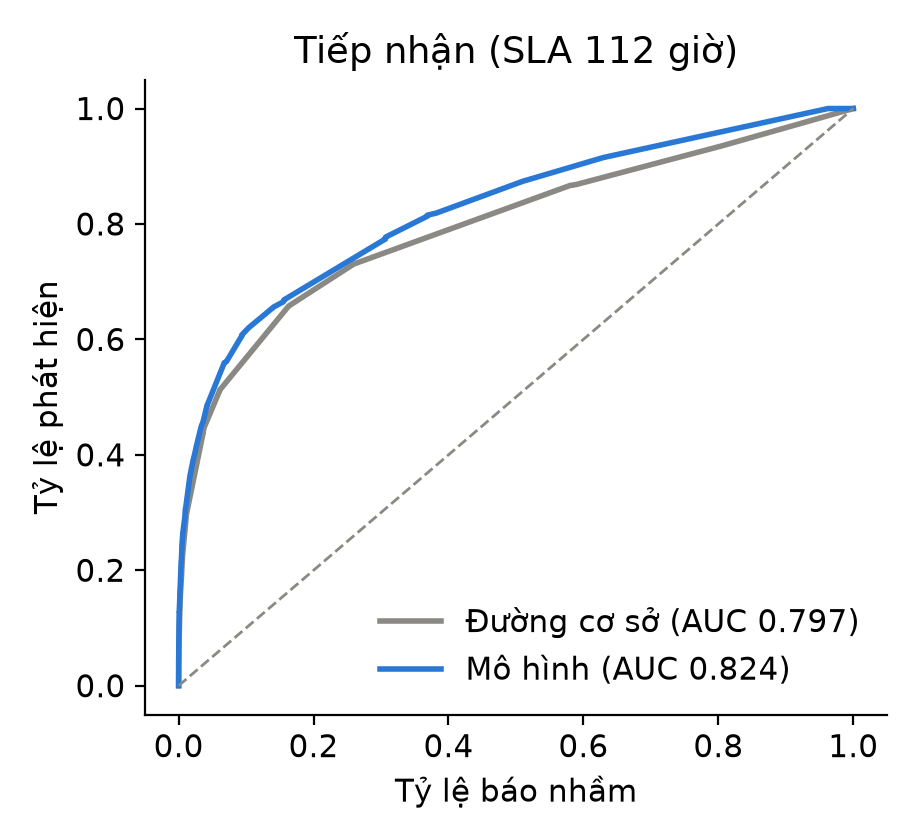
\includegraphics[width=0.36\textwidth]{roc_tiep_nhan.png}\hspace{0.06\textwidth}
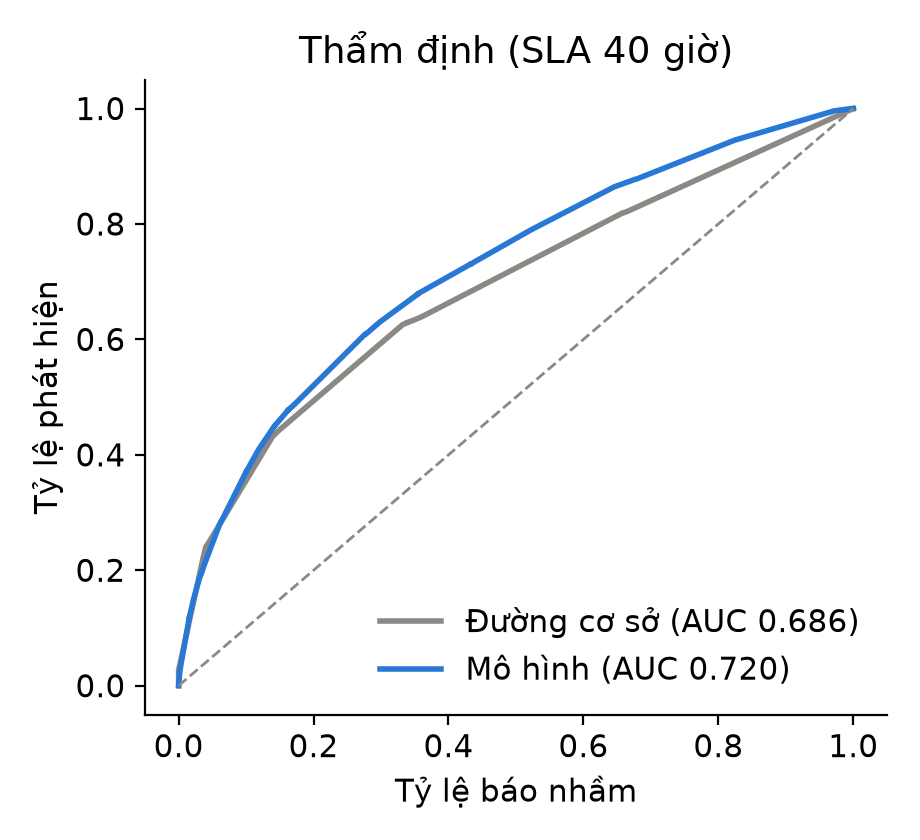
\includegraphics[width=0.36\textwidth]{roc_tham_dinh.png}
\caption{Đường ROC của mô hình đang dùng và của đường cơ sở trên tập kiểm tra: (a) Tiếp nhận, SLA 112 giờ; (b) Thẩm định, SLA 40 giờ. Đường nét đứt là đoán bừa.}
\label{fig:roc}
\end{figure*}

\begin{figure*}[t]
\centering
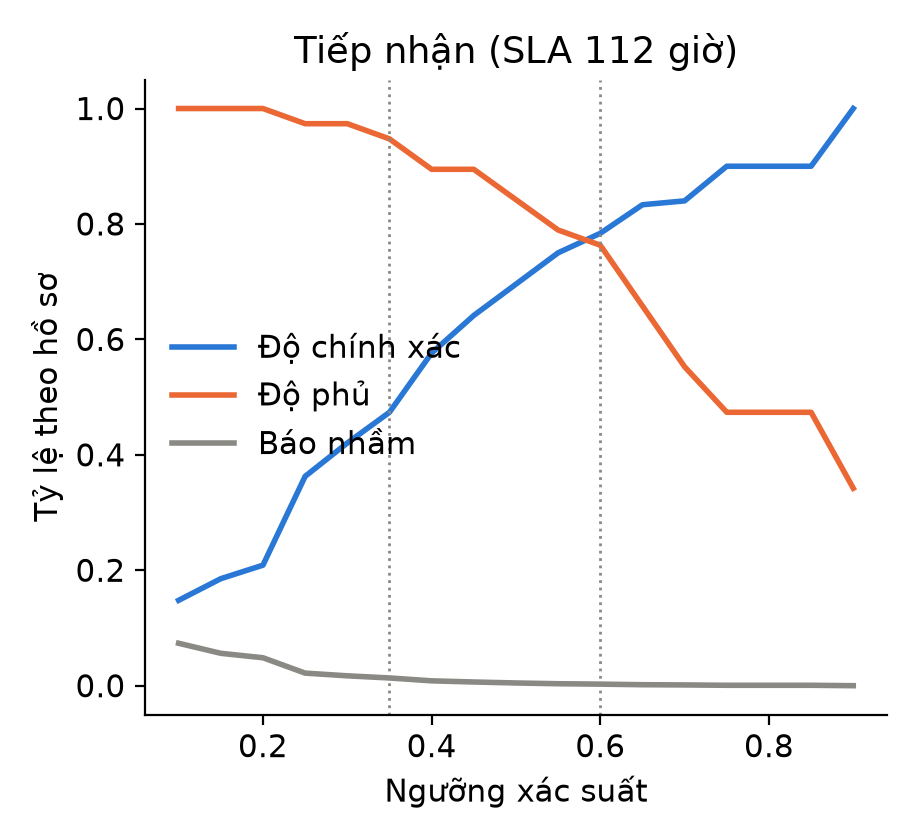
\includegraphics[width=0.36\textwidth]{nguong_tiep_nhan.png}\hspace{0.06\textwidth}
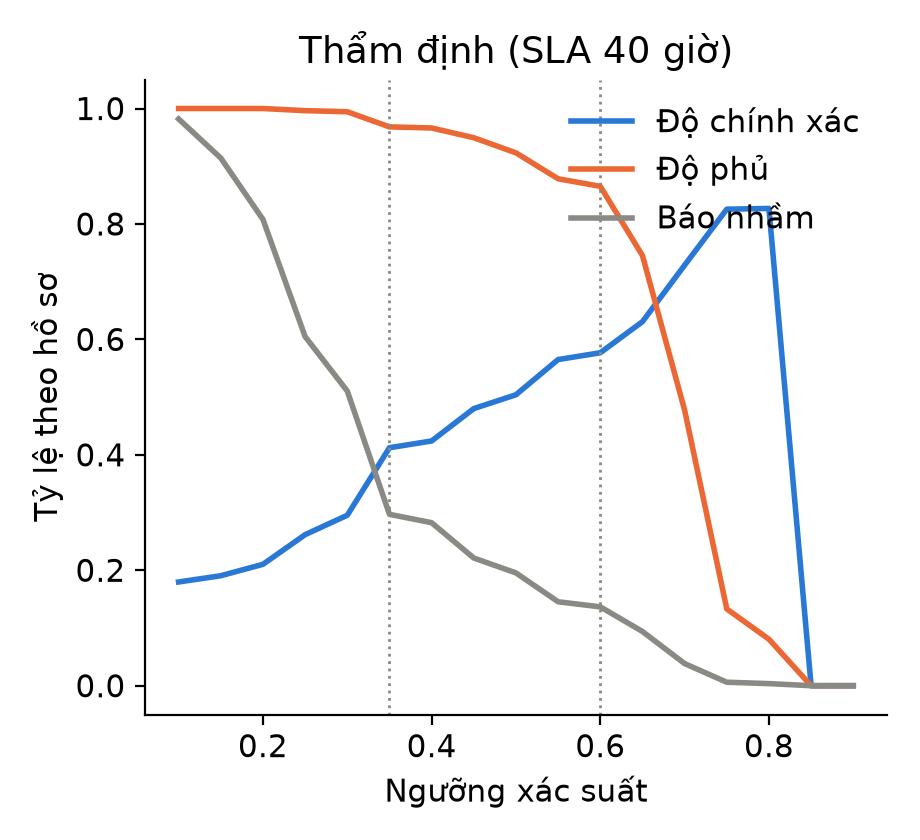
\includegraphics[width=0.36\textwidth]{nguong_tham_dinh.png}
\caption{Độ chính xác, độ phủ và tỷ lệ báo nhầm theo ngưỡng xác suất: (a) Tiếp nhận; (b) Thẩm định. Hai đường chấm đứng là ngưỡng 0,35 và 0,60.}
\label{fig:thr}
\end{figure*}

\begin{table}[t]
\caption{Kết quả trên tập kiểm tra, lần chạy chính thức (dữ liệu mô phỏng). KTC: khoảng tin cậy}
\label{tab:result}
\centering
\begin{tabular}{|l|c|c|}
\hline
Chỉ số & Tiếp nhận & Thẩm định \\
\hline
AUC mô hình / cơ sở & 0,824 / 0,797 & 0,720 / 0,687 \\
Hiệu AUC [KTC 95\%] & +0,027 [$-$0,006; 0,059] & +0,034 [0,020; 0,047] \\
Brier mô hình / theo tỷ lệ chung & 0,0280 / 0,0353 & 0,1765 / 0,2048 \\
Khẩn: độ chính xác / độ phủ & 78,4\% / 76,3\% & 57,7\% / 86,5\% \\
Khẩn: báo nhầm hồ sơ đúng hạn & 0,3\% & 13,7\% \\
AUC lúc vào công đoạn & 0,557 & 0,634 \\
\hline
\end{tabular}
\end{table}

\subsection{So sánh thuật toán}
Bảng~\ref{tab:algo} so sánh năm phương án trên cùng dữ liệu. Ba thuật toán học máy cho kết quả gần nhau: ở Tiếp nhận chênh lệch nằm trong độ lệch chuẩn giữa các hạt giống, còn ở Thẩm định Random Forest nhỉnh hơn hồi quy logistic khoảng 0,01 AUC và có log-loss tốt hơn (0,5285 so với 0,5416). Việc giữ hồi quy logistic cho Thẩm định vì đơn giản và dễ giải thích là hợp lý, nhưng không phải phương án tốt nhất về số liệu; Random Forest không nằm trong các ứng viên lúc chọn. Luật ngưỡng gần như bằng đường cơ sở học máy (0,795 và 0,793 ở Tiếp nhận), nên mốc so sánh đáng kể thực chất là đồng hồ SLA.

\begin{table}[t]
\caption{So sánh thuật toán, trung bình $\pm$ độ lệch chuẩn của năm hạt giống}
\label{tab:algo}
\centering
\small
\begin{tabular}{|l|c|c|c|c|}
\hline
 & \multicolumn{2}{c|}{Tiếp nhận} & \multicolumn{2}{c|}{Thẩm định} \\
Phương án & AUC & Brier & AUC & Brier \\
\hline
Luật ngưỡng & 0,795$\pm$0,001 & --- & 0,686$\pm$0,003 & --- \\
Chỉ đồng hồ SLA & 0,793$\pm$0,003 & 0,0297 & 0,686$\pm$0,003 & 0,1798 \\
Hồi quy logistic & 0,802$\pm$0,007 & 0,0293 & 0,716$\pm$0,004 & 0,1794 \\
Random Forest & 0,806$\pm$0,013 & 0,0280 & 0,726$\pm$0,005 & 0,1748 \\
Gradient Boosting & 0,813$\pm$0,017 & 0,0284 & 0,719$\pm$0,010 & 0,1768 \\
\hline
\end{tabular}
\end{table}

\subsection{Bóc tách thành phần}
Bảng~\ref{tab:abl} bỏ lần lượt từng thành phần của mô hình đang dùng. Hai kết quả đáng chú ý. Thứ nhất, sức dự báo đến từ đặc trưng vận hành (tải cán bộ, số vòng bổ sung, hàng chờ, số người thẩm quyền, số lần làm rõ): bỏ nhóm này AUC giảm 0,026 ở Tiếp nhận và 0,023 ở Thẩm định. Thứ hai, thông tin về hồ sơ và doanh nghiệp (số tiền, ngành, doanh thu\ldots) không giúp dự báo và ở Tiếp nhận còn gây nhiễu (bỏ đi AUC tăng từ 0,813 lên 0,829); điều này khớp với bộ mô phỏng, nơi các đặc trưng đó không được cài làm nguyên nhân gây chậm. Hiệu chỉnh đẳng điệu giảm sai số hiệu chỉnh ở Thẩm định (ECE 0,0188 so với 0,0240) nhưng không ích ở Tiếp nhận (0,0105 so với 0,0067) vì chỉ có vài chục hồ sơ trễ để học bộ hiệu chỉnh.

\begin{table}[t]
\caption{Bóc tách thành phần, AUC trung bình $\pm$ độ lệch chuẩn}
\label{tab:abl}
\centering
\small
\begin{tabular}{|l|c|c|}
\hline
Biến thể & Tiếp nhận & Thẩm định \\
\hline
Đầy đủ & 0,813$\pm$0,017 & 0,716$\pm$0,004 \\
Bỏ thông tin hồ sơ & 0,829$\pm$0,006 & 0,714$\pm$0,002 \\
Bỏ đặc trưng vận hành & 0,788$\pm$0,022 & 0,693$\pm$0,006 \\
Bỏ giờ từ thao tác gần nhất & 0,809$\pm$0,017 & 0,713$\pm$0,003 \\
Không hiệu chỉnh & 0,816$\pm$0,016 & 0,718$\pm$0,003 \\
Chỉ đồng hồ SLA & 0,791$\pm$0,004 & 0,686$\pm$0,003 \\
\hline
\end{tabular}
\end{table}

\subsection{SLA là đầu vào}
Để kiểm tra thiết kế ``SLA là đầu vào'', so sánh với mô hình huấn luyện ở một mức SLA cố định (112 giờ cho Tiếp nhận, 40 giờ cho Thẩm định) rồi đo ở mức SLA khác (Hình~\ref{fig:sla}). Khi định mức đổi, mô hình cố định dự báo sai về xác suất: điểm Brier ở Tiếp nhận SLA 48 giờ là 0,270 so với 0,178 của mô hình nhận biết SLA, và ở Thẩm định SLA 24 giờ là 0,309 so với 0,233. AUC của mô hình cố định cũng thấp hơn ở Tiếp nhận (0,567 so với 0,693 ở SLA 48). Đây là bằng chứng ủng hộ rõ nhất cho thiết kế này, vì nó cho phép quản trị viên đổi định mức mà không phải huấn luyện lại.

\begin{figure}[t]
\centering
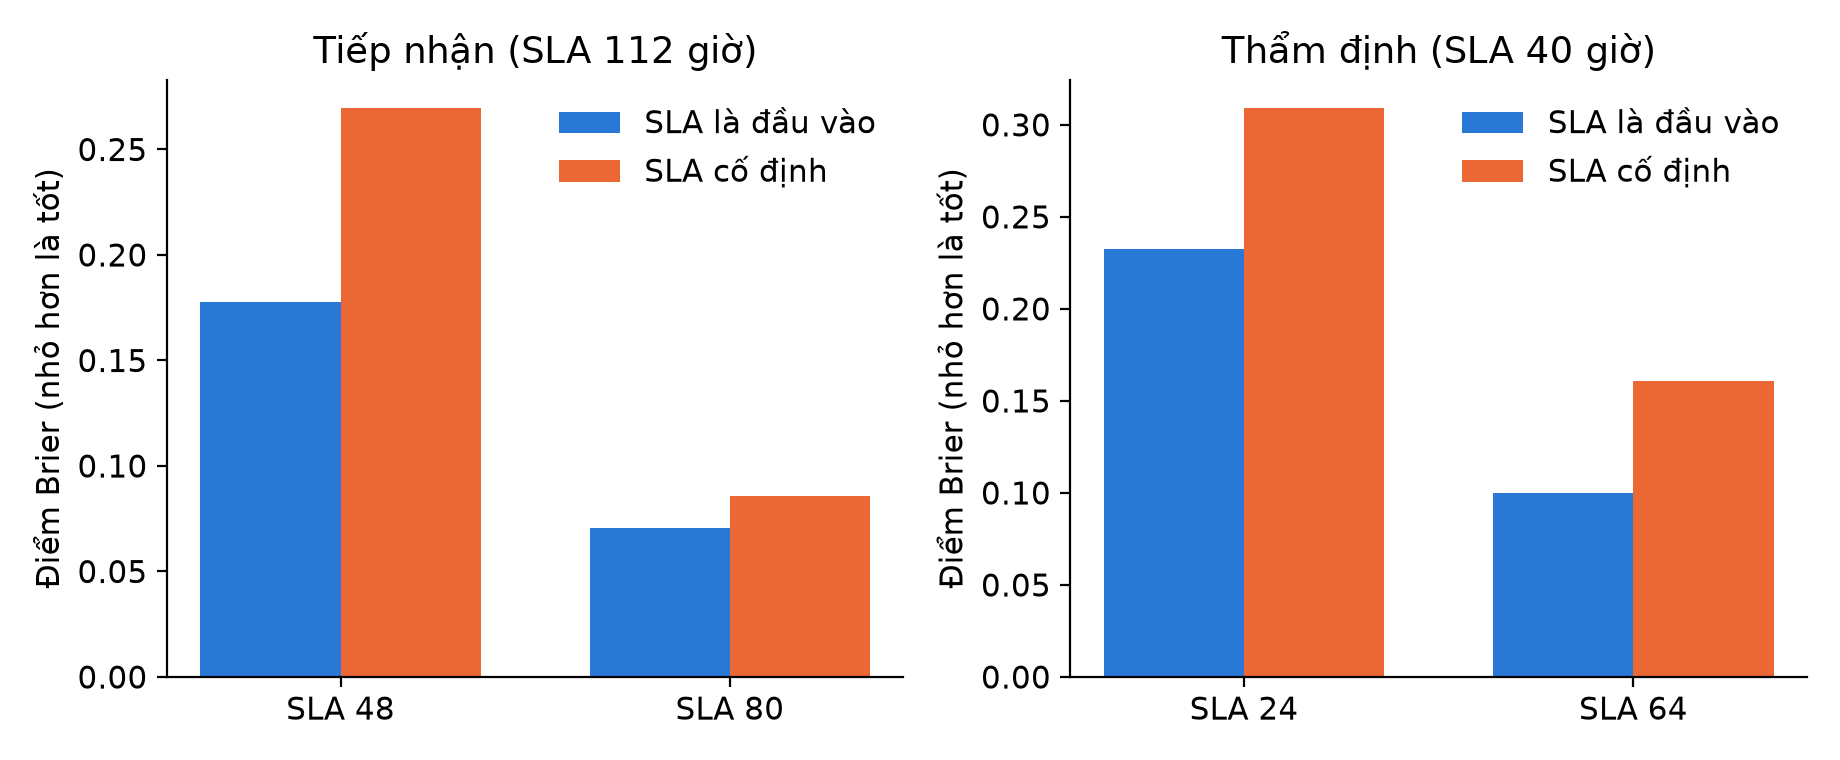
\includegraphics[width=\columnwidth]{sla_nhan_biet.png}
\caption{Điểm Brier (nhỏ hơn là tốt) khi đo ở mức SLA khác mức đã huấn luyện: mô hình nhận SLA làm đầu vào so với mô hình huấn luyện ở SLA cố định.}
\label{fig:sla}
\end{figure}

\subsection{Hiệu chỉnh xác suất}
Hình~\ref{fig:calib} so sánh xác suất mô hình dự báo với tỷ lệ hồ sơ thực sự trễ. Cả hai công đoạn bám sát đường chéo, tức là con số 0,6 gần đúng ứng với 60\% hồ sơ thực sự trễ. Thẩm định hơi nằm dưới đường chéo ở xác suất cao, nghĩa là mô hình dự báo nhỉnh hơn thực tế khoảng 3--6 điểm phần trăm.

\begin{figure}[t]
\centering
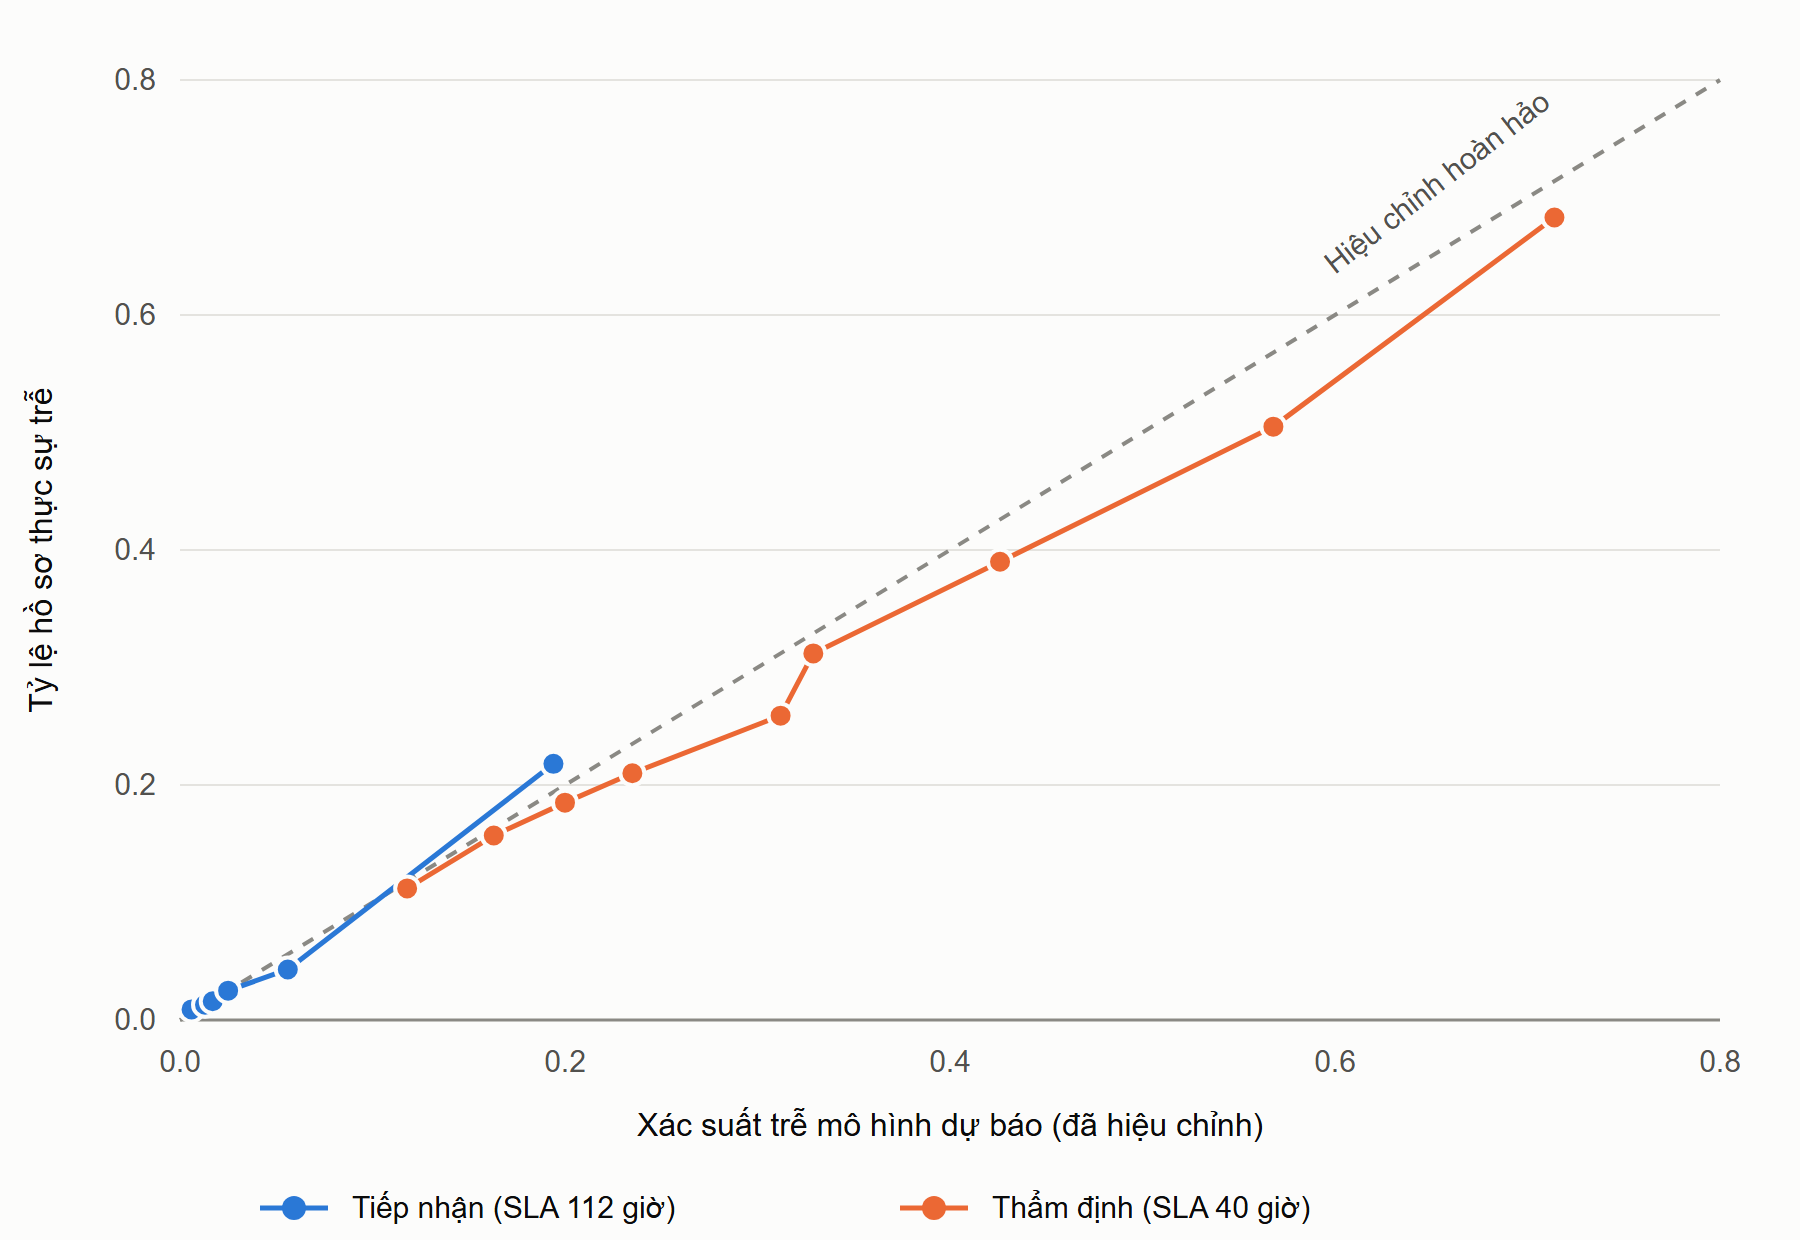
\includegraphics[width=\columnwidth]{hinh-5-2-calibration.png}
\caption{Xác suất mô hình dự báo so với tỷ lệ hồ sơ thực sự trễ trên tập kiểm tra; đường nét đứt là hiệu chỉnh hoàn hảo.}
\label{fig:calib}
\end{figure}

\subsection{Trần lý thuyết và độ nhạy với giả định mô phỏng}
Vì dữ liệu được sinh ra, ta biết ba biến ẩn mà mô hình không được thấy. Chạy lại bộ mô phỏng để lấy các biến này (sinh lại khớp 20\,000/20\,000 hồ sơ) rồi cho mô hình thấy chúng, AUC tăng lên 0,894 ở Tiếp nhận (Gradient Boosting) và 0,776 ở Thẩm định (hồi quy logistic). Tính theo phần AUC vượt mức đoán bừa (0,5):
\begin{equation}
\rho=\frac{\mathrm{AUC}_{\text{quan sát}}-0{,}5}{\mathrm{AUC}_{\text{biến ẩn}}-0{,}5},
\end{equation}
mô hình đang dùng đạt $\rho\approx 0{,}82$ ở Tiếp nhận và $\rho\approx 0{,}80$ ở Thẩm định so với mô hình thấy được cả biến ẩn. Nói cách khác, AUC khiêm tốn chủ yếu do thông tin quan sát được tại thời điểm dự báo có hạn, không phải do thuật toán yếu; ngay cả khi biết biến ẩn, Thẩm định cũng chỉ đạt khoảng 0,78 vì thời gian xử lý từng bước vốn có độ ngẫu nhiên cao.

Để biết kết luận có phụ thuộc vào giả định của người mô phỏng hay không, bảy bộ tham số được thử (giảm hoặc tăng một nửa độ lệch của biến ẩn, thời gian xử lý $\pm$20\%, độ nhạy với hàng chờ $\times$0,5 và $\times$1,5), mỗi bộ sinh lại 20\,000 hồ sơ. Ở Thẩm định, mô hình hơn đường cơ sở trong cả bảy kịch bản (từ +0,026 đến +0,061 AUC). Ở Tiếp nhận, mô hình hơn ở SLA 80 giờ trong cả bảy kịch bản (+0,020 đến +0,044) và ở SLA 112 giờ trong sáu kịch bản; kịch bản còn lại (biến ẩn giảm một nửa, chỉ còn 174 dòng trễ) cho hiệu $-$0,019. Kết luận về Thẩm định vì vậy vững, còn kết luận về Tiếp nhận chỉ vững ở mức ``hơi hơn''.

\subsection{Lý do giải thích}
Trên các dòng có xác suất từ 10\% trở lên, mọi dòng ở Tiếp nhận và 73,5\% dòng ở Thẩm định có ít nhất một lý do. Phân loại các đặc trưng theo cơ chế trong bộ mô phỏng, 70,1\% (Tiếp nhận) và 75,4\% (Thẩm định) lý do rơi vào nhóm có tác động trực tiếp lên thời gian xử lý, và không lý do nào nằm ngoài phân loại. Có ba hạn chế: lý do ``thời gian đã dùng'' xuất hiện ở phần lớn dòng nên ít thông tin; ở Tiếp nhận khoảng 20\% lý do chỉ vào số tiền đề nghị, yếu tố mà bóc tách cho thấy không giúp dự báo; và ở Thẩm định 21\% lý do thuộc nhóm đại diện (chủ yếu là giờ đã tốn ở Tiếp nhận), thay cho độ phức tạp ẩn chứ không phải nguyên nhân. Đánh giá này chỉ đo mức khớp với cơ chế mô phỏng, chưa đo việc cán bộ có hiểu và hành động theo lý do hay không.

\subsection{Kiểm chứng tích hợp}
Bộ kiểm thử tự động của máy chủ nghiệp vụ gồm 498 kiểm thử, tất cả đạt ở lần chạy gần nhất. Bộ này bao gồm các kịch bản gắn với dự báo: hồ sơ lập tại quầy được chấm điểm ngay và lỗi của dịch vụ dự báo không làm hỏng việc tạo hồ sơ; mỗi lần trình tờ trình hoặc yêu cầu làm rõ làm mới dự báo và thao tác lặp lại không sinh dòng trùng; lượt quét định kỳ dừng sớm mà không gây lỗi khi dịch vụ dự báo liên tục thất bại; và chỉ dự báo hiện hành của đúng công đoạn mới được tính vào các chỉ số tổng hợp. Cả năm dịch vụ (giao diện, máy chủ, cơ sở dữ liệu, dịch vụ dự báo, hộp thư thử) ở trạng thái hoạt động khi kiểm tra, và dịch vụ dự báo báo đã nạp mô hình phiên bản v4.0.

Về độ trễ, riêng mô hình cho một hồ sơ mất trung vị 7,1 ms (Tiếp nhận) và 2,5 ms (Thẩm định) trên máy phát triển; qua giao diện lập trình của dịch vụ là 9,3 ms và 41,3 ms (trung vị, 300 lần gọi). Thẩm định chậm hơn vì ca thử có xác suất cao nên phải tính thêm phần lý do giải thích (nhiều lần dự báo với từng yếu tố bị thay thế). Cả hai đủ nhanh cho việc chấm theo sự kiện và theo lượt quét định kỳ. Việc kiểm chứng với người dùng thật (cán bộ có tin và hành động theo cảnh báo hay không) chưa được thực hiện.

% ============================================================
\section{Hạn chế}
% ============================================================
Toàn bộ số liệu đo trên dữ liệu mô phỏng, chất lượng với hồ sơ thực chưa biết; các tham số giả định chưa được cán bộ thực xác nhận. Năng lực dự báo chỉ hơn đường cơ sở khoảng 0,03 AUC, chưa có ý nghĩa thống kê ở Tiếp nhận (chỉ 38 hồ sơ trễ trong tập kiểm tra), và gần như không phân biệt được ngay lúc hồ sơ vào công đoạn. Thông tin về hồ sơ và doanh nghiệp không giúp dự báo trong bộ mô phỏng này, và phần lý do giải thích chưa được kiểm chứng với người dùng. Báo nhầm ở Thẩm định còn cao. Huấn luyện chỉ với 2 hoặc 3 người thẩm quyền nên số lượng khác là ngoại suy. Số tài liệu chờ kiểm tra ở Tiếp nhận chỉ là xấp xỉ vì hệ thống chưa lưu số lượng, và dự báo phụ thuộc lịch làm việc đã nạp. Hai ngưỡng cảnh báo là lựa chọn của dự án, chưa được tối ưu hóa theo chi phí thực của chi nhánh. Cuối cùng, kết quả đo độ trễ lấy trên một máy phát triển, chưa phải môi trường vận hành thực.

% ============================================================
\section{Kết luận và hướng phát triển}
% ============================================================
Bài báo trình bày một hệ thống quản lý quy trình vay SME tích hợp dự báo nguy cơ trễ SLA theo từng công đoạn. Mô hình nhận SLA làm đầu vào nên đổi định mức không phải huấn luyện lại, xác suất được hiệu chỉnh và mỗi cảnh báo có lý do kèm theo; dịch vụ dự báo tách rời nên nghiệp vụ không bị ảnh hưởng khi dịch vụ gặp sự cố. Trên dữ liệu mô phỏng, mô hình đạt AUC 0,824 ở Tiếp nhận (trung bình năm lần chia 0,813) và 0,720 ở Thẩm định. Mức hơn đường cơ sở chỉ biết đồng hồ SLA có ý nghĩa thống kê ở Thẩm định (+0,034) và vững trước thay đổi giả định mô phỏng, nhưng ở Tiếp nhận (+0,027) chưa đủ bằng chứng. Bằng chứng mạnh nhất cho thiết kế là việc coi SLA như một đầu vào giữ xác suất đúng khi định mức đổi. Kết quả được tái lập chính xác trên một môi trường độc lập.

Hướng phát triển: thu thập dữ liệu vận hành thực của chi nhánh để huấn luyện lại và hiệu chỉnh ngưỡng; khảo sát cán bộ tín dụng để xác nhận các tham số giả định; lưu số lượng tài liệu bổ sung thay cho giá trị xấp xỉ; và đánh giá tác động của cảnh báo lên tỷ lệ hồ sơ trễ thực tế.

\section*{Lời cảm ơn}
Nhóm tác giả đã thiết kế nghiên cứu, xây dựng và kiểm thử hệ thống, chạy các thực nghiệm và đối chiếu số liệu trong các bảng. Claude (Anthropic) \cite{claude2026} được sử dụng dưới sự giám sát của nhóm để hỗ trợ soạn thảo văn bản và viết các tập lệnh thực nghiệm; mọi nội dung đã được nhóm rà soát. Nhóm tác giả chịu toàn bộ trách nhiệm về bài báo này.

\begin{thebibliography}{00}
\bibitem{teinemaa2019} I. Teinemaa, M. Dumas, M. La Rosa, and F. M. Maggi, ``Outcome-oriented predictive process monitoring: Review and benchmark,'' \textit{ACM Trans. Knowl. Discov. Data}, 2019. doi: 10.1145/3301300.

\bibitem{verenich2019} I. Verenich, M. Dumas, M. La Rosa, F. M. Maggi, and I. Teinemaa, ``Survey and cross-benchmark comparison of remaining time prediction methods in business process monitoring,'' \textit{ACM Trans. Intell. Syst. Technol.}, vol. 10, no. 4, pp. 34:1--34:34, 2019.

\bibitem{tax2017} N. Tax, I. Verenich, M. La Rosa, and M. Dumas, ``Predictive business process monitoring with LSTM neural networks,'' in \textit{Proc. 29th Int. Conf. Advanced Information Systems Engineering (CAiSE)}, Essen, Germany, 2017, pp. 477--492. doi: 10.1007/978-3-319-59536-8\_30.

\bibitem{senderovich2015} A. Senderovich, M. Weidlich, A. Gal, and A. Mandelbaum, ``Queue mining for delay prediction in multi-class service processes,'' \textit{Inf. Syst.}, vol. 53, pp. 278--295, 2015. doi: 10.1016/j.is.2015.03.010.

\bibitem{niculescu2005} A. Niculescu-Mizil and R. Caruana, ``Predicting good probabilities with supervised learning,'' in \textit{Proc. 22nd Int. Conf. Machine Learning (ICML)}, 2005, pp. 625--632. doi: 10.1145/1102351.1102430.

\bibitem{guo2017} C. Guo, G. Pleiss, Y. Sun, and K. Q. Weinberger, ``On calibration of modern neural networks,'' in \textit{Proc. 34th Int. Conf. Machine Learning (ICML)}, PMLR 70, 2017, pp. 1321--1330.

\bibitem{brier1950} G. W. Brier, ``Verification of forecasts expressed in terms of probability,'' \textit{Mon. Weather Rev.}, vol. 78, no. 1, pp. 1--3, 1950.

\bibitem{friedman2001} J. H. Friedman, ``Greedy function approximation: A gradient boosting machine,'' \textit{Ann. Statist.}, vol. 29, no. 5, pp. 1189--1232, Oct. 2001. doi: 10.1214/aos/1013203451.

\bibitem{pedregosa2011} F. Pedregosa \textit{et al.}, ``Scikit-learn: Machine learning in Python,'' \textit{J. Mach. Learn. Res.}, vol. 12, pp. 2825--2830, 2011.

\bibitem{bpic2012} B. F. van Dongen, ``BPI Challenge 2012,'' 4TU.ResearchData, dataset, 2012. doi: 10.4121/uuid:3926db30-f712-4394-aebc-75976070e91f. [Online]. Available: https://data.4tu.nl/articles/\_/12689204/1. Accessed on: Nov. 13, 2026.

\bibitem{efron1979} B. Efron, ``Bootstrap methods: Another look at the jackknife,'' \textit{Ann. Statist.}, vol. 7, no. 1, pp. 1--26, 1979.

\bibitem{wilson1927} E. B. Wilson, ``Probable inference, the law of succession, and statistical inference,'' \textit{J. Amer. Statist. Assoc.}, vol. 22, no. 158, pp. 209--212, 1927.

\bibitem{claude2026} Anthropic, ``Claude (Sonnet 5.5),'' AI system, 2026. [Online]. Available: https://www.anthropic.com/claude. Accessed on: Nov. 14, 2026.
\end{thebibliography}

\end{document}
